\documentclass{article}

\usepackage{graphicx}

\begin{document}
\newpage
   \vspace*{\stretch{1.0}}
   \begin{center}
      \Large\textbf{Earth 436B Thesis}\\
      \large\textit{John Lawson}
   \end{center}
   \vspace*{\stretch{2.0}}

\newpage





\DTLloaddb{result}{data/bothNonZero_withinSeventyFivePercent_intervals.csv}
\newcommand{\result}[1]{%
    \dtlgetrowforvalue{result}{\dtlcolumnindex{result}{id}}{#1}%
    % read variables into commands
\dtlgetentryfromcurrentrow{\id}{1}
\dtlgetentryfromcurrentrow{\name}{2}
\dtlgetentryfromcurrentrow{\startValue}{3}
\dtlgetentryfromcurrentrow{\endValue}{4}

% use commands in text
\text{\startValue} to \text{\endValue} cm/century

%
}


\section{Abstract}

The ground surface underlying the Laurentian Great Lakes is currently undergoing vertical adjustment
 after being depressed by the weight of an ice sheet formed in the most recent glacial period during the Wisconsonian.
 The rate of glacial isostatic adjustment (GIA) varies by location, and strongly influences the flow of water
 in the Laurentian Great Lakes (LGL) as the inclination of the ground surface changes. Previous attempts to 
 estimate the rate of GIA between sites used geologically recent water gauge data from the
 past 200 years in order to measure the rate of GIA. In contrast, by
 inferring GIA from measurements of the water level in the geological record over the past 5000 years,
 a more accurate estimate of the long term process of GIA can be obtained. These measurements are
 made by measuring the elevation of a subsurface sedimentary contact relating to
 past lake levels,which are then age dated with optically stimulated luminescence
 (OSL) to provide an age for sediments. Elevation and age data are then compiled
 to create site paleohydrographs for each location around the lake basin.\\
 
 The focus of this paper is to analyze the data compiled by Johnston et al, 2014
 which measured past elevation of shorelines by interpreting water levels recorded
 in the sediment record. Each site paleohydrograph
 is now extended between points where the data was measured directly, then subtracted
 from one data point to a modelled elevation in order to create a
 plot of relative elevation over time. Once this is done, the rate of change per unit
 time is obtained from a linear regression, representing an estimate of the value
 of GIA between each pair of sites. This process is repeated for
 all possible combinations of the four sites used, 
 Grand Traverse Bay (GTB), Au Train Bay (ATB), Batchawana Bay (BATB), and Tahquamenon Bay (TAHB).\\
 
 
 
 The results of this process were in strong agreement at the 95 \% confidence level for GIA rates obtained from
 forward and reverse regressions for the combination of ATB-BATB (23.5 to 31 cm/century) and
 BATB-TAHB (11 to 17 cm/century). Agreement was also seen at the 95 \% confidence level for GTB-TAHB (anywhere from -3 to 8.5 cm/century),
 ATB-GTB (9 to 13 cm/century) and ATB-TAHB (19.5 to 29 cm/century).

\newpage

\section{Introduction}
 The Earths crust rests on top of the mantle, its elevation rising and falling
 with the amount of mass weighing on it. During glacial periods, a significant portion
 of the water on earth is transferred in form from water in the Oceans to glacial ice,
 weighing down the continental crust. This causes the crust to ride lower in elevation,
 a change which is quickly reversed when the weight is removed as the ice sheets melt.
 This vertical motion of the crust while returning to its previous position is known
 as glacial isostatic adjustment (GIA).\\
 
 This process of isostatic rebound has implications for the routes that the flow
 of water on the Earths surface takes; the "tilting" of the surface caused by 
 uneven rates of GIA in different locations may open or close locations along basins,
 causing some rivers and lake outlets to close, while potentially opening others.
 Additionally, the change in "tilt" has potential to change shorelines of existing
 basins, which has implications for property assessment, structural projections, etc.\\
 
 In order to project the future impact of this process on the Great Lakes Basin,
 an estimate of the historical rate of GIA is needed. This estimate is obtained by
 comparing the elevation of the water mark at two different locations around a basin, and
 observing how this difference changes over time. The elevation of the water can be inferred
 by a variety of indicators in the sediment record, in this case, beach deposits known
 as strandplain sequences are used, their ages determined by optically stimulated
 luminescence (OSL) dating. This raw data is presented in Figure \ref{fig:rawData}.\\
\begin{figure}[h]
	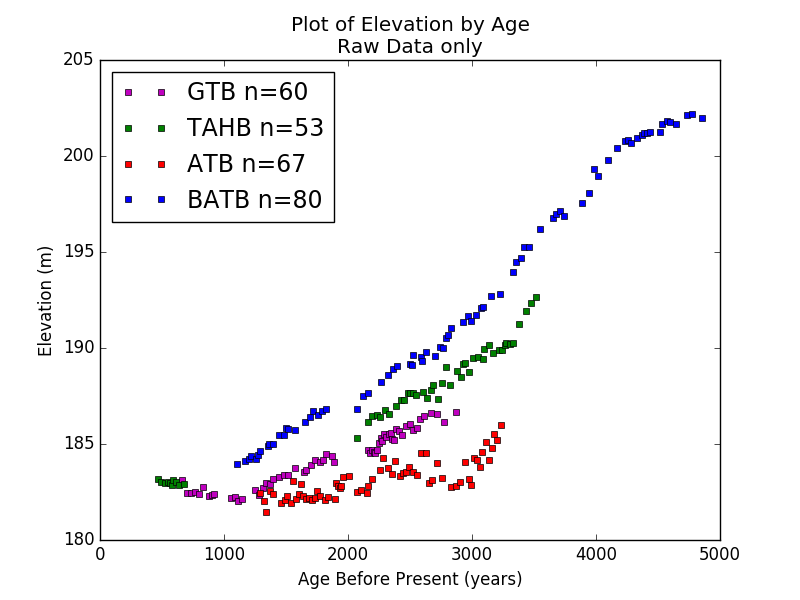
\includegraphics[width=1.1\linewidth]{data/theDataRaw.png}
	\caption{Current day elevation of relict shorelines with respect to time before present over the last 5000 years. Strandplain sites Au Train Bay, Michigan (ATB), Batchawana Bay, Ontario (BATB), Tahquamenon Bay, Michigan (TAHB), and Grand Traverse Bay, Michigan (GTB) surrounding Lake Superior are plotted individually. Data from Johnston et al, (2012)}
	\label{fig:rawData}
\end{figure} 
%\begin{figure}[h]
	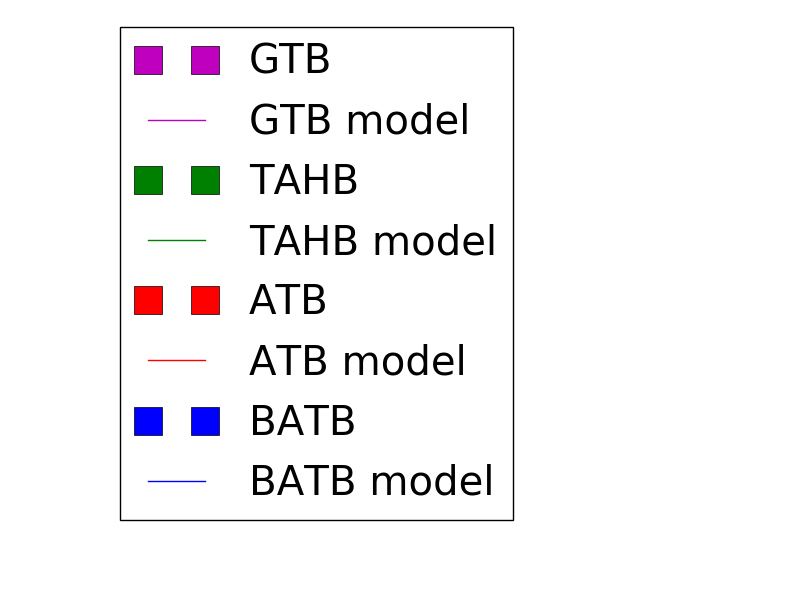
\includegraphics[width=0.40\textwidth]{data/legendary.png}
	%\makebox[\textwidth]{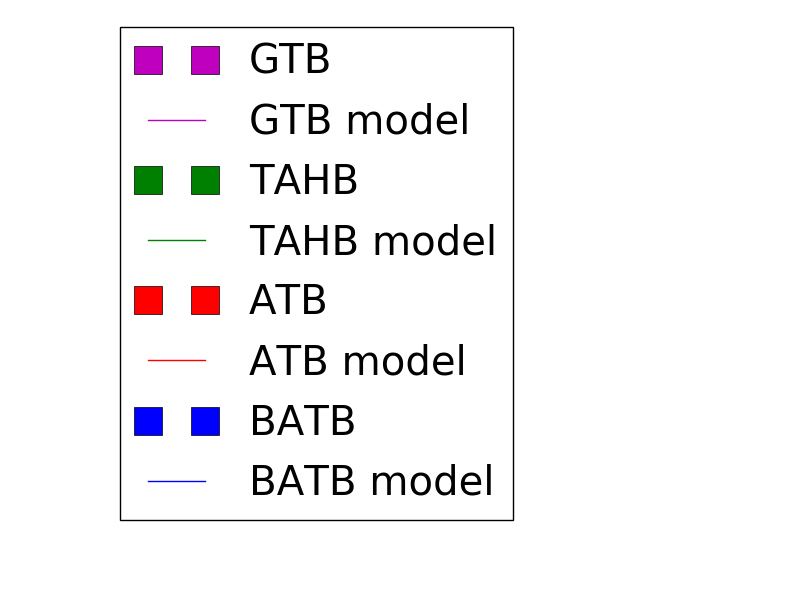
\includegraphics[width=\paperwidth]{data/legendary.png}}
	%\caption{Site Legend}
	%\label{fig:rdmLegend}
\end{figure}



\newpage 
 
 Given that none of the datasets have elevations sampled
 at the same times, an estimate of elevation is needed for times where one dataset
 has a data point present, but the other does not. This estimate 
 (the modelled elevation) is created by using linear interpolation between datapoints,
 represented as a solid line between points in Figure \ref{fig:rawDataWithModel}.\\
\begin{figure}[h]
	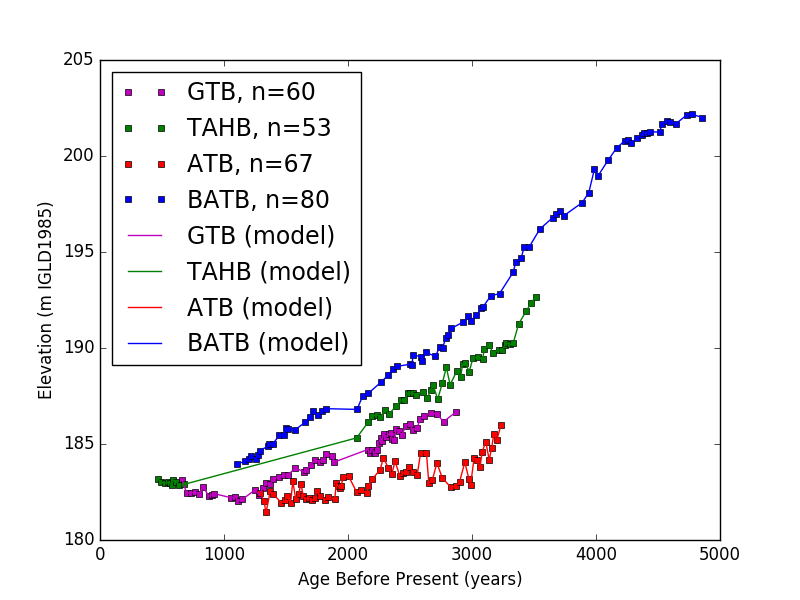
\includegraphics[width=\linewidth]{data/theData.png}
	\caption{Water surface elevation with respect to time before present, modelled}
	\label{fig:rawDataWithModel}
\end{figure}
\newpage
%\begin{figure}[h]
	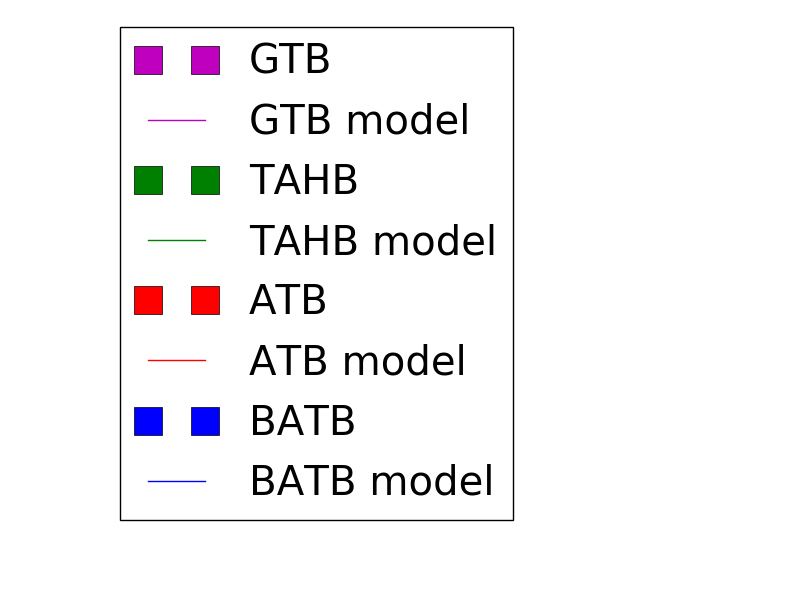
\includegraphics[width=0.40\textwidth]{data/legendary.png}
	%\makebox[\textwidth]{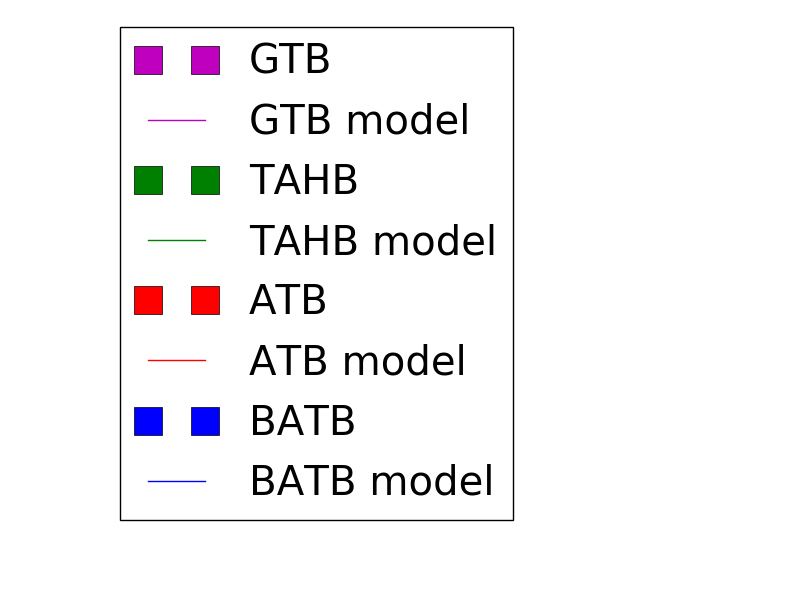
\includegraphics[width=\paperwidth]{data/legendary.png}}
	%\caption{Site Legend}
	%\label{fig:rdmLegend}
\end{figure}


 
\newpage
\section{Previous Work} 
Mainville \& Craymer (2005) used water gauge data collected around the LGL over the past 150 years to
 create monthly means of water level. Differences in these values between sites
 were then plotted against time to calculate a rate of elevation change between
 sites over time (This value is interpreted to represent the impact of the GIA
 process on the crust underlying the LGL, even though the actual process extends
 over a much longer timescale than that of the data collection). Combinations of sites were shown to produce
 inconsistent results, so a second method using a least squares adjustment process was used,
 removing some monthly mean outliers which plotted at or beyond some arbitrary residual distance away 
 from the linear regression line in the vertical (elevation) axis. 
 This process was repeated with each new linear regression on the remaining data
 points until none remained "too far away" from
 the final regression line. A third, and ultimately optimal method for calculating
 GIA was developed by
 Mainville \& Craymer in their 2005 paper, this time computing velocity at a given
 month from the difference between a
 the monthly water level mean and an reference water level for the epoch that the 
 month is found in (this 
 reference level being adjusted for epoch
 and site biases). This elevation difference is then divided by the time difference
 between the start of the epoch and the month that was measured, calculating a rate
 of GIA for the month measured. Their findings with this method showed a general agreement with the post glacial
 ICE-3G global model of GIA at that time, while the ICE-4G model developed by Peltier
 was shown to underestimate the relative difference in vertical movement across
 the span of the Great Lakes (Mainville \& Craymer, 2005).\\ \\
Johnston et al. (2012) attempted to provide a value for GIA in the LGL with
 better accuracy than previous estimates calculated using water
 gauge data.
 
In order to accomplish this, the data used to measure the process of
 GIA needed to extend over a much longer timescale. In this method, water
 levels were inferred from the elevation of relict shorelines in beach ridge
 strandplains from the late Holocene sediment record surrounding Lake Superior.
 Ages for each elevation were inferred from age dating samples from these beach
 deposits (known as strandplain sequences) using
 optically stimulated luminescence (OSL) age dating. Johnston et al (2012) differed from
 Mainville \& Craymer (2005), in that data collected for the 2012 paper using OSL
 age dating did not have
 elevations sampled at the same points in time for calculation of relative
 rates. As a result, Johnston et al (2012) the elevation vs time data was modelled with a linear
 regression for each site, the difference in slopes of each regression representing the GIA rate
 between sites. Individual regressions were further created per site
 for a series of four ranges of time related to lake level phases, namely the Nipissing,
 Algoma, Sault, and Sub-Sault (Johnston et al, 2012). The results reported from this process
 are summarized in Figure \ref{fig:jj2012Grid}. \\
 
 \begin{figure}[t]
	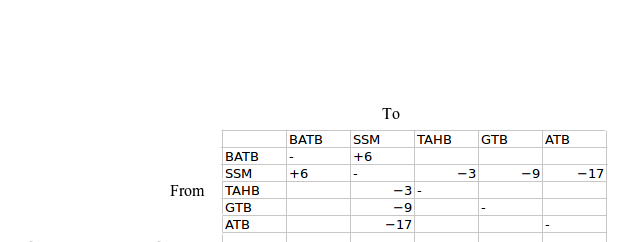
\includegraphics[width=0.9\linewidth]{jjGrid.png}
	\caption{GIA values reported by Johnston et al 2012. All values are in cm/century.}
	\label{fig:jj2012Grid}
 \end{figure}
 % need to ask JJ about JJ 2012, bottom of page 3, divergence of intercepts
 






\newpage
\begin{figure}[t]
	\makebox[\textwidth]{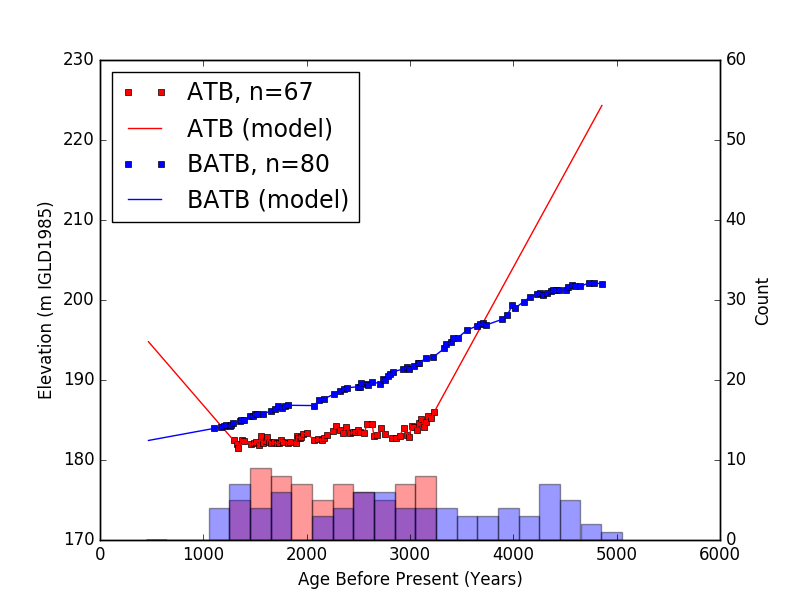
\includegraphics[width=0.72\paperwidth]{data/ATB-BATB_DataAndModel.png}}
	\caption{ATB-BATB raw data with linear interpolation model}
	\label{fig:data_ATBxBATB}
\end{figure}
\newpage

\begin{figure}[t]
	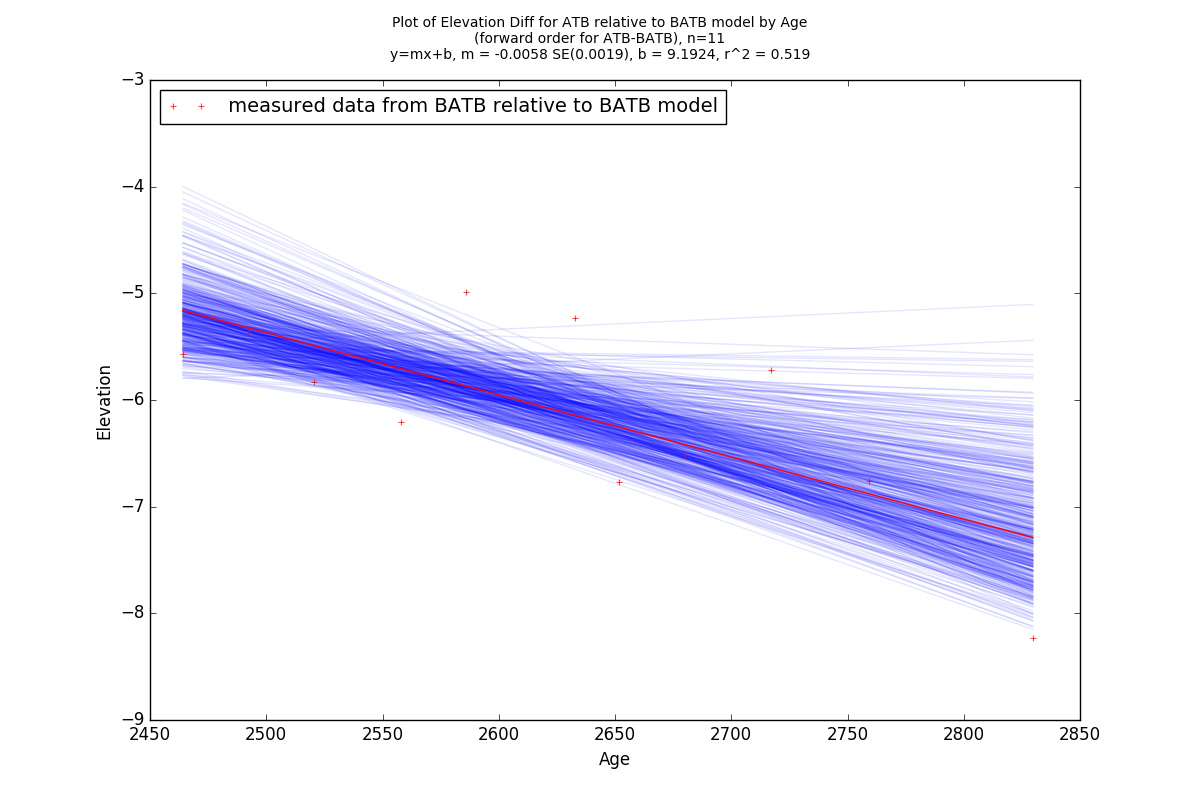
\includegraphics[width=0.9\linewidth]{data/gias/theGIA_ATB_relative_to_BATB.png}
	\caption{Differences in elevation measured from the ATB data to the ATB model}
	\label{fig:gias_ATBxBATB}
\end{figure}
\newpage


\begin{figure}[t]
	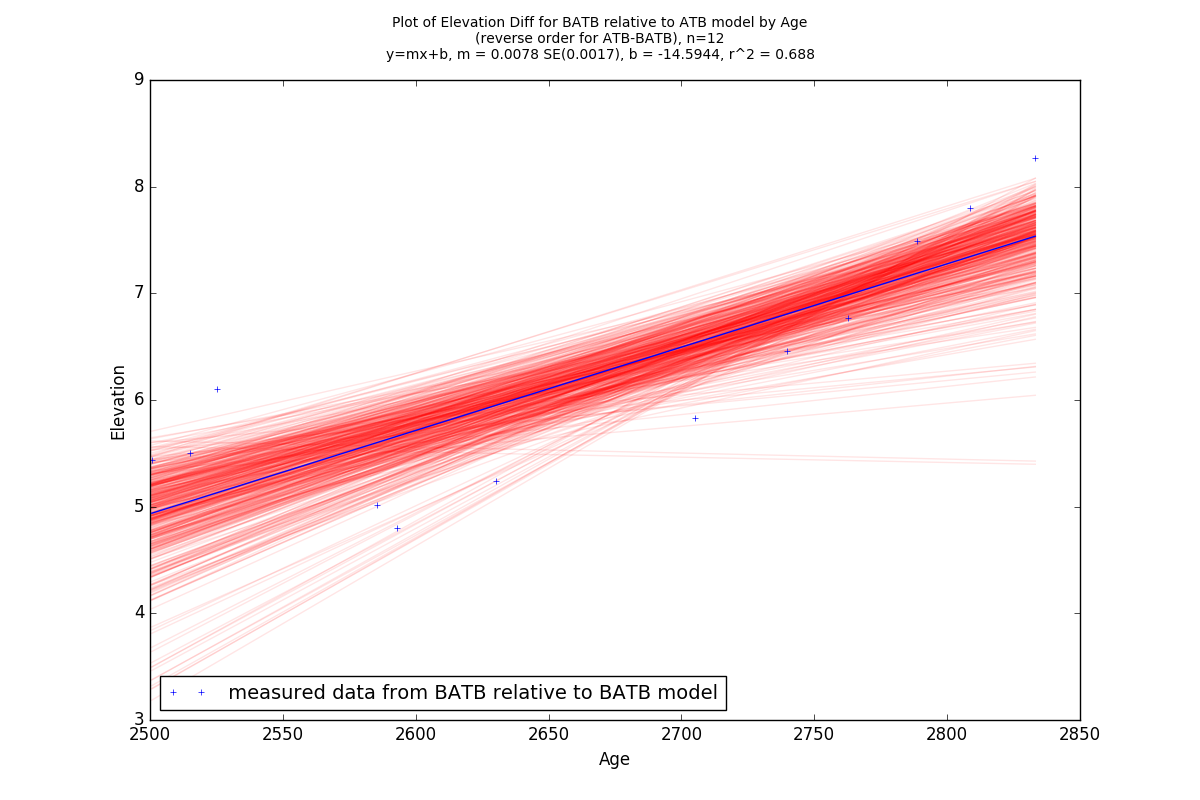
\includegraphics[width=0.9\linewidth]{data/gias/theGIA_BATB_relative_to_ATB.png}
	\caption{Differences in elevation measured from the BATB data to the ATB model}
	\label{fig:gias_BATBxATB}
\end{figure}
\newpage
% this desperately needs to be done as a loop



\begin{figure}[h]
	\makebox[\textwidth]{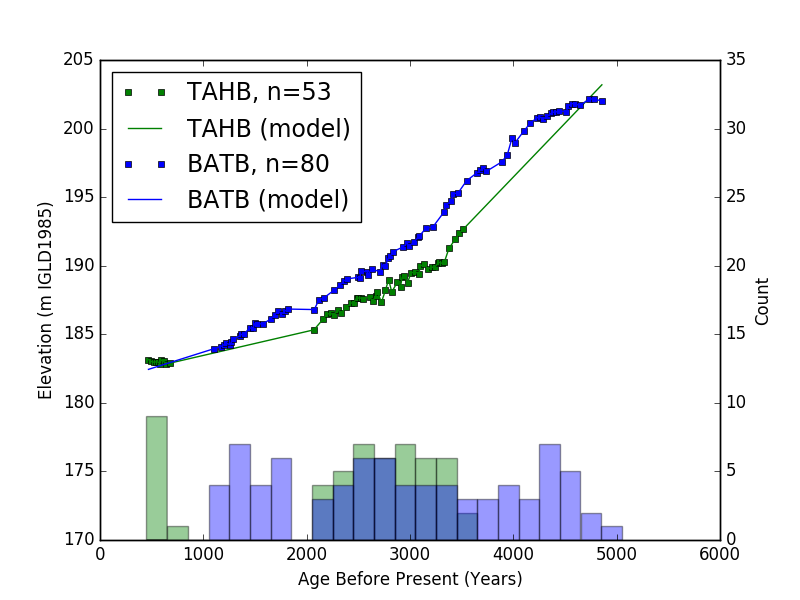
\includegraphics[width=0.72\paperwidth]{data/TAHB-BATB_DataAndModel.png}}
	\caption{TAHB-BATB raw data with linear interpolation model}
	\label{fig:data_TAHBxBATB}
\end{figure}
\newpage

\begin{figure}[h]
	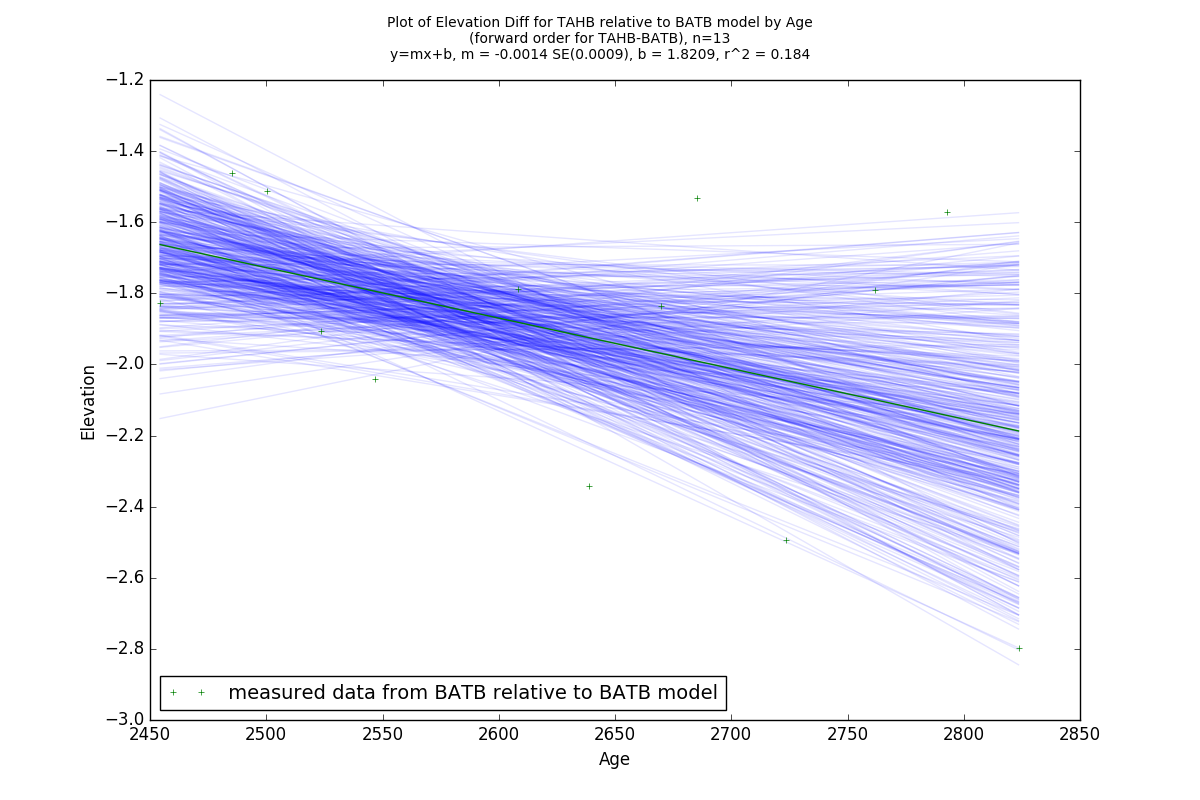
\includegraphics[width=0.9\linewidth]{data/gias/theGIA_TAHB_relative_to_BATB.png}
	\caption{Differences in elevation measured from the TAHB data to the BATB model}
	\label{fig:gias_TAHBxBATB}
\end{figure}
\newpage


\begin{figure}[h]
	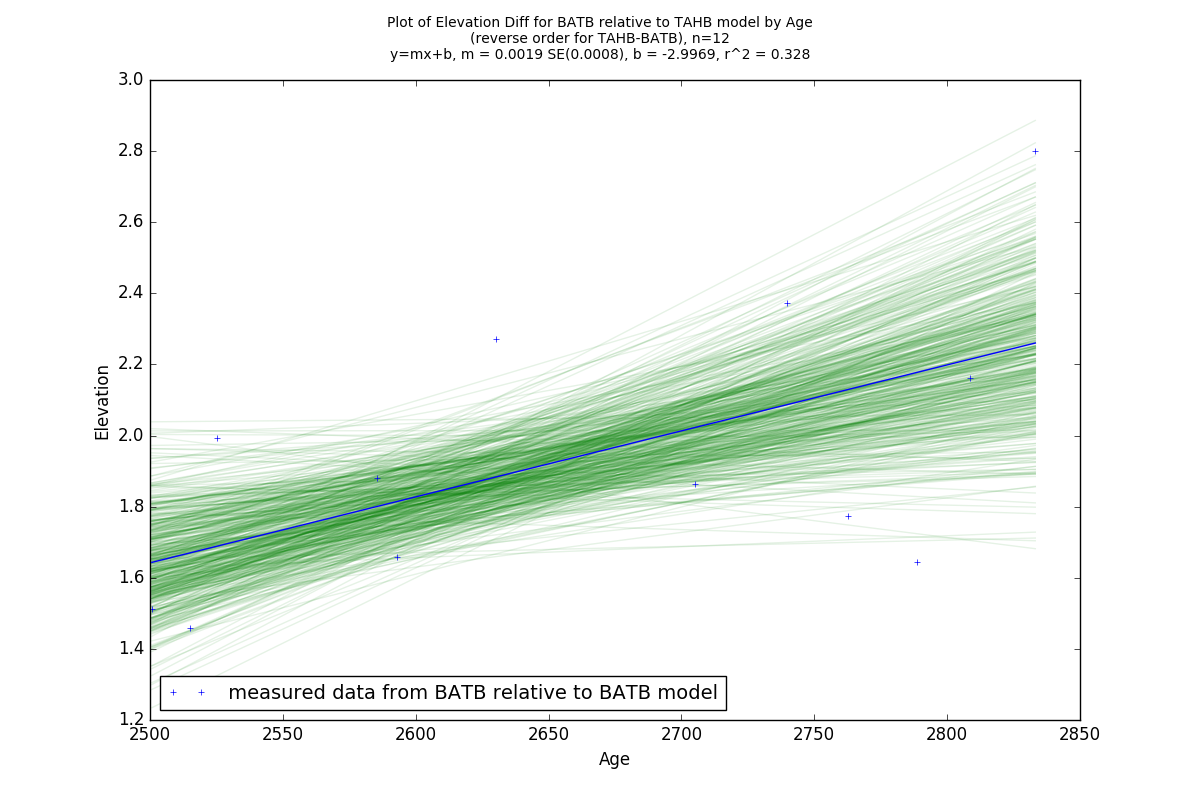
\includegraphics[width=0.9\linewidth]{data/gias/theGIA_BATB_relative_to_TAHB.png}
	\caption{Differences in elevation measured from the BATB data to the TAHB model}
	\label{fig:gias_BATBxTAHB}
\end{figure}
\newpage








\begin{figure}[h]
	\makebox[\textwidth]{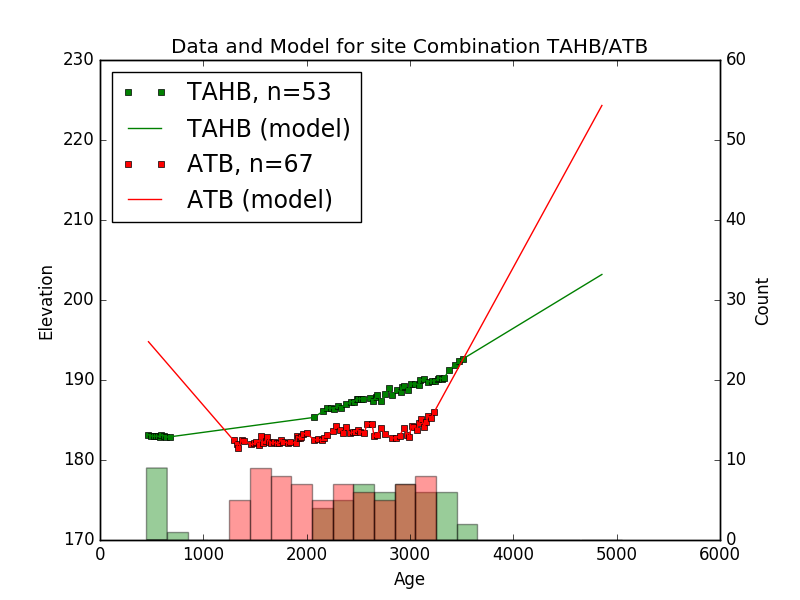
\includegraphics[width=0.72\paperwidth]{data/TAHB-ATB_DataAndModel.png}}
	\caption{TAHB-ATB raw data with linear interpolation model}
	\label{fig:data_TAHBxATB}
\end{figure}
\newpage

\begin{figure}[h]
	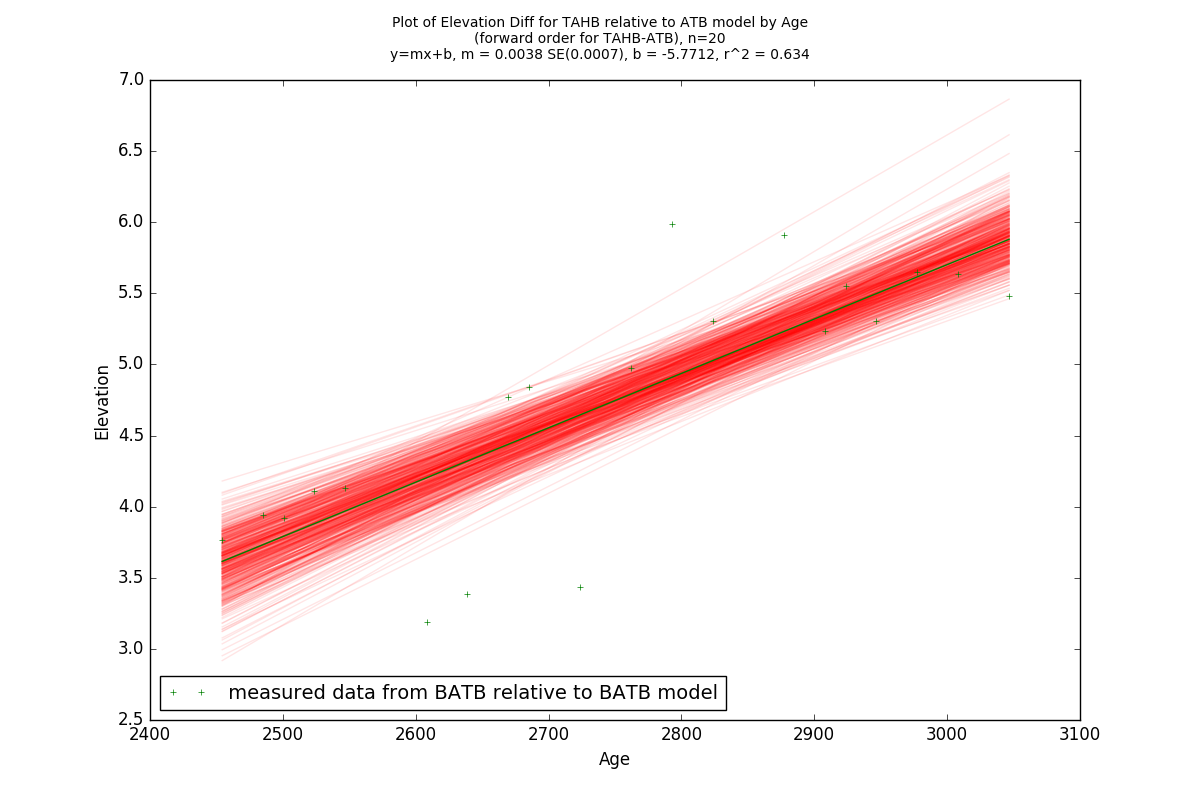
\includegraphics[width=0.9\linewidth]{data/gias/theGIA_TAHB_relative_to_ATB.png}
	\caption{Differences in elevation measured from the TAHB data to the ATB model}
	\label{fig:gias_TAHBxATB}
\end{figure}
\newpage


\begin{figure}[h]
	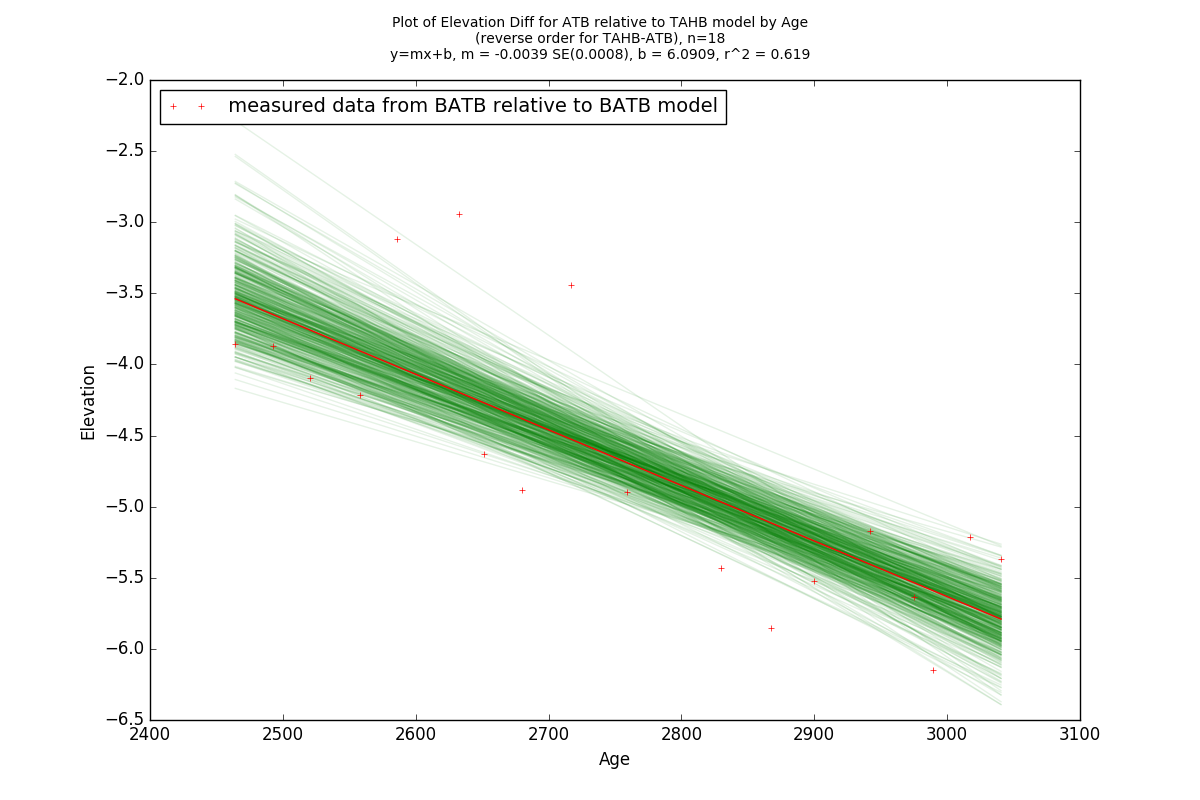
\includegraphics[width=0.9\linewidth]{data/gias/theGIA_ATB_relative_to_TAHB.png}
	\caption{Differences in elevation measured from the ATB data to the TAHB model}
	\label{fig:gias_ATBxTAHB}
\end{figure}
\newpage






\begin{figure}[h]
	\makebox[\textwidth]{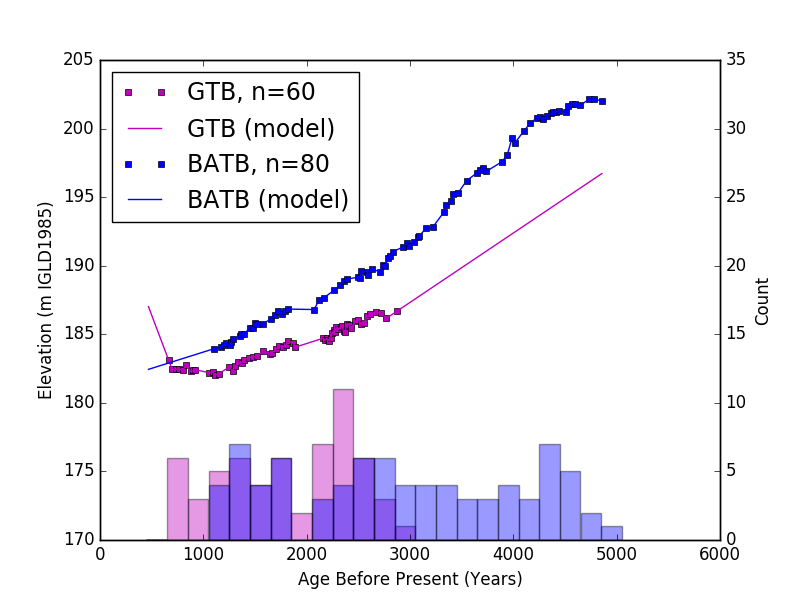
\includegraphics[width=0.72\paperwidth]{data/GTB-BATB_DataAndModel.png}}
	\caption{GTB-BATB raw data with linear interpolation model}
	\label{fig:data_GTBxBATB}
\end{figure}
\newpage

\begin{figure}[h]
	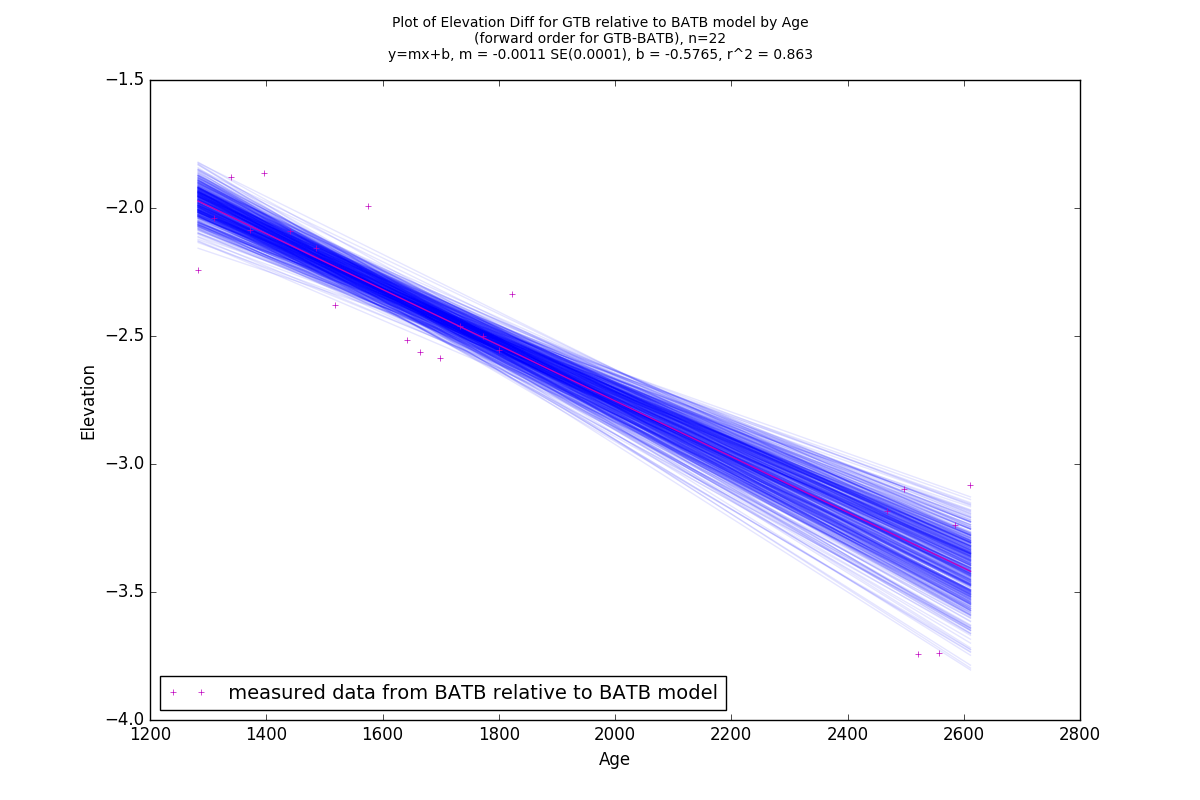
\includegraphics[width=0.9\linewidth]{data/gias/theGIA_GTB_relative_to_BATB.png}
	\caption{Differences in elevation measured from the GTB data to the BATB model}
	\label{fig:gias_GTBxBATB}
\end{figure}
\newpage


\begin{figure}[h]
	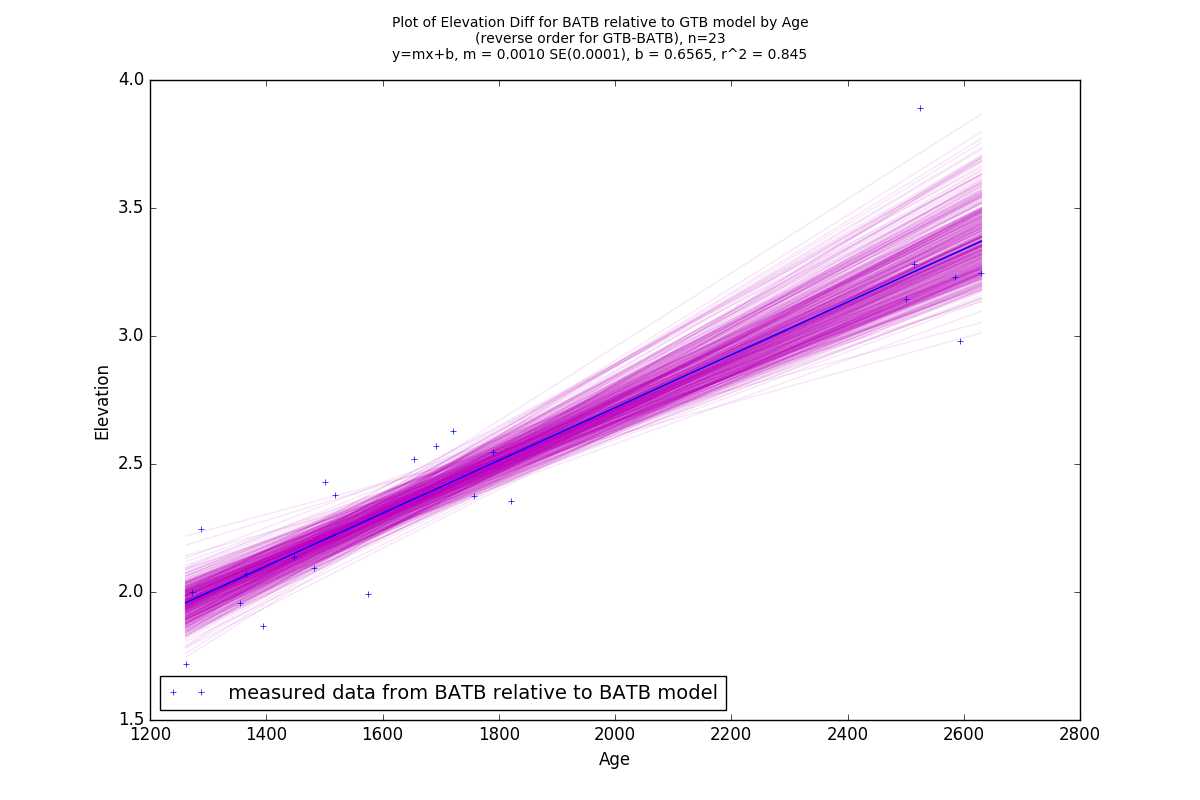
\includegraphics[width=0.9\linewidth]{data/gias/theGIA_BATB_relative_to_GTB.png}
	\caption{Differences in elevation measured from the BATB data to the GTB model}
	\label{fig:gias_BATBxGTB}
\end{figure}
\newpage









\begin{figure}[h]
	\makebox[\textwidth]{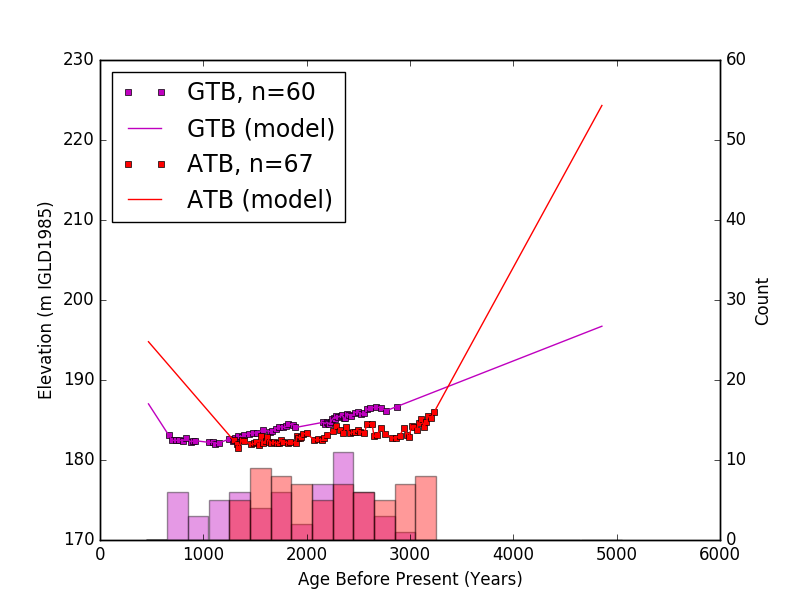
\includegraphics[width=0.72\paperwidth]{data/GTB-ATB_DataAndModel.png}}
	\caption{GTB-ATB raw data with linear interpolation model}
	\label{fig:data_GTBxATB}
\end{figure}
\newpage

\begin{figure}[h]
	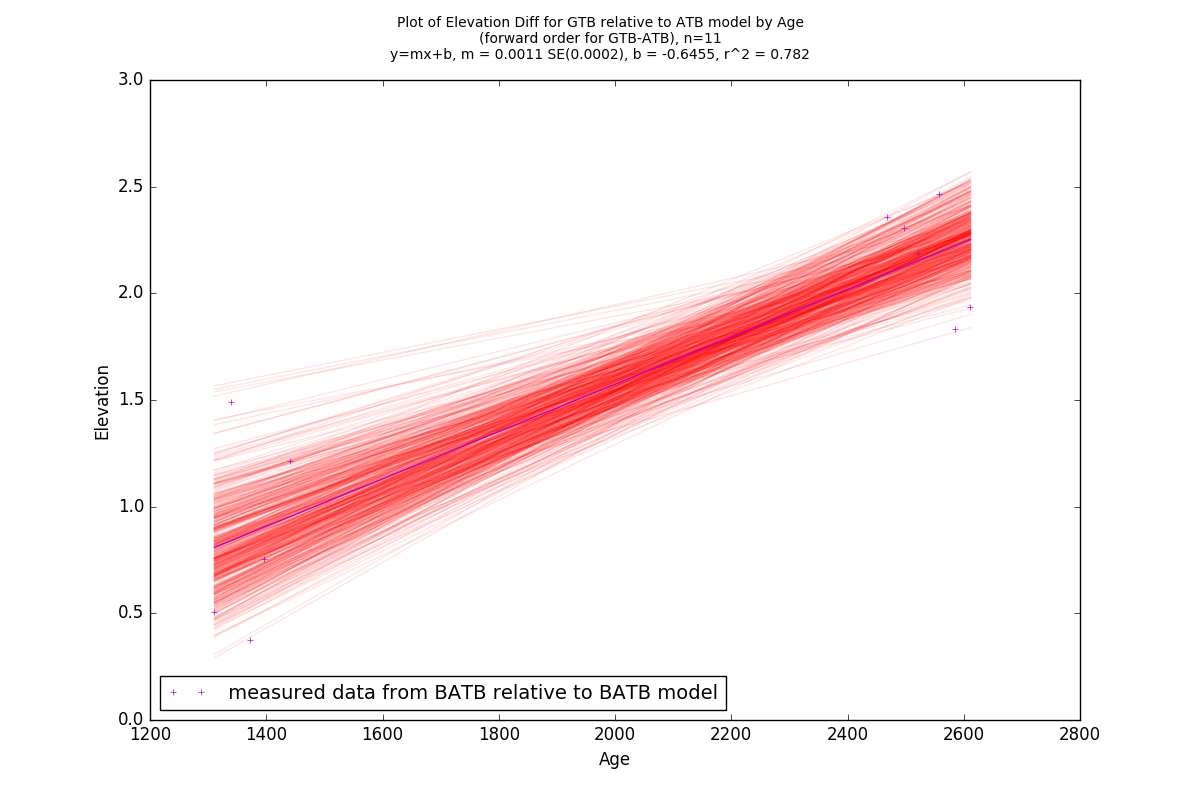
\includegraphics[width=0.9\linewidth]{data/gias/theGIA_GTB_relative_to_ATB.png}
	\caption{Differences in elevation measured from the GTB data to the ATB model}
	\label{fig:gias_GTBxATB}
\end{figure}
\newpage


\begin{figure}[h]
	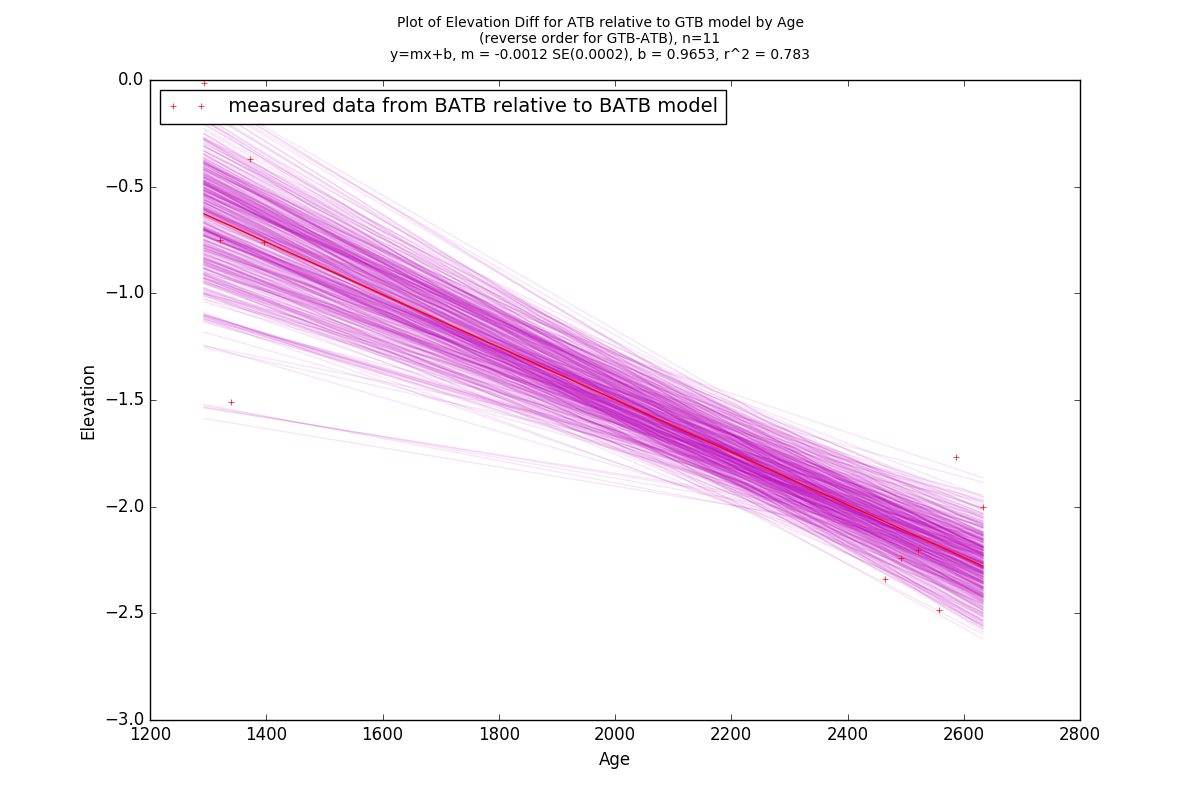
\includegraphics[width=0.9\linewidth]{data/gias/theGIA_ATB_relative_to_GTB.png}
	\caption{Differences in elevation measured from the ATB data to the GTB model}
	\label{fig:gias_ATBxGTB}
\end{figure}
\newpage










\begin{figure}[h]
	\makebox[\textwidth]{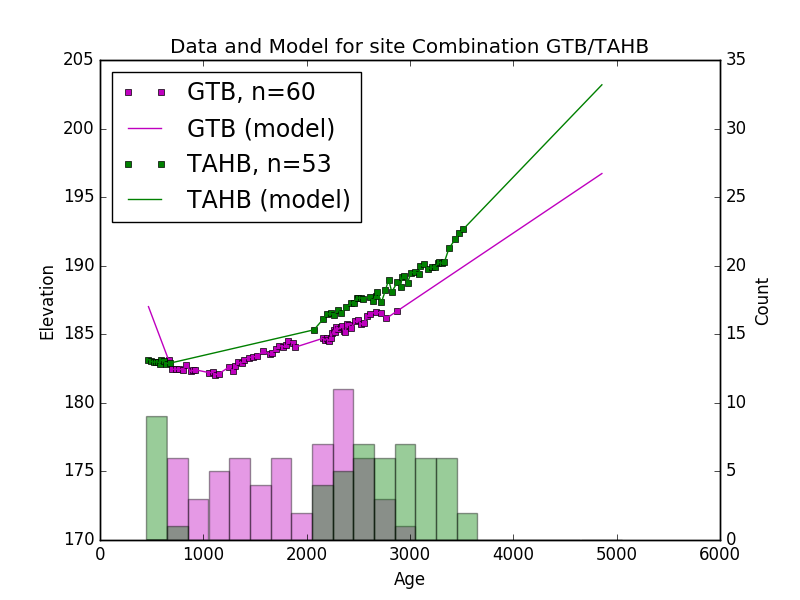
\includegraphics[width=0.72\paperwidth]{data/GTB-TAHB_DataAndModel.png}}
	\caption{GTB-TAHB raw data with linear interpolation model}
	\label{fig:data_GTBxTAHB}
\end{figure}
\newpage

\begin{figure}[h]
	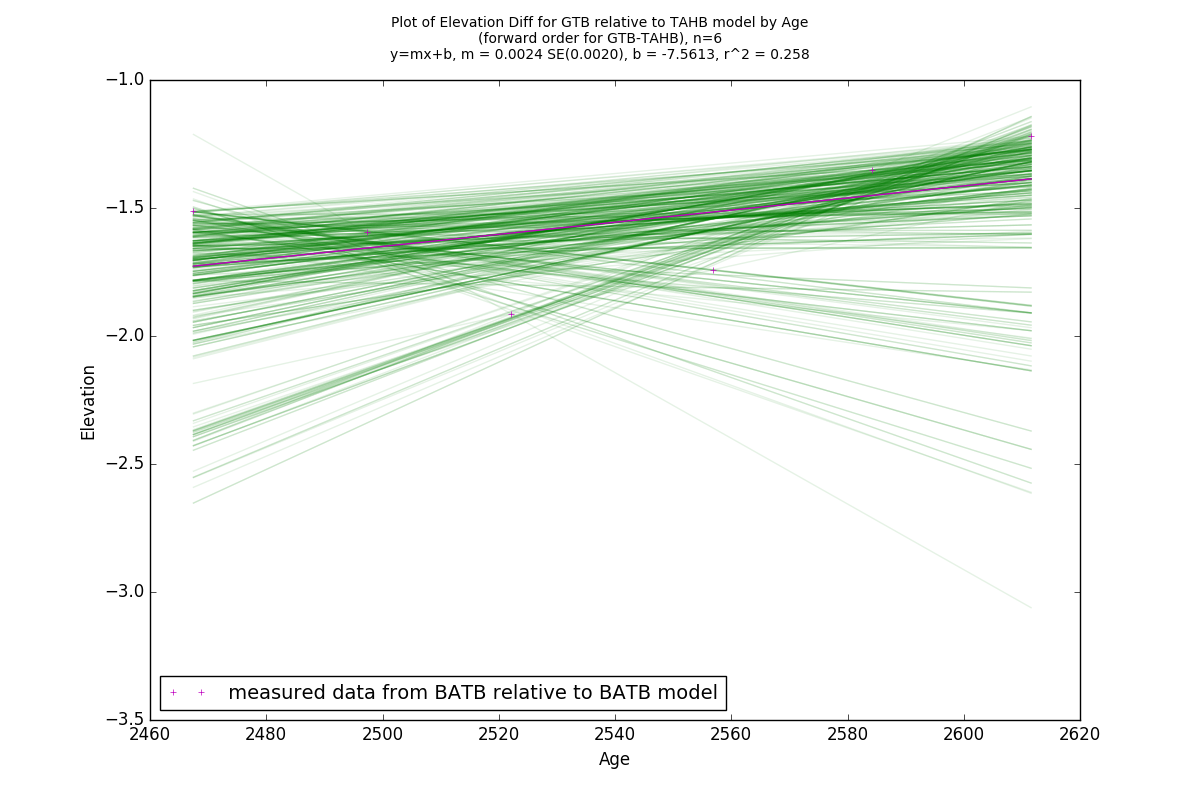
\includegraphics[width=0.9\linewidth]{data/gias/theGIA_GTB_relative_to_TAHB.png}
	\caption{Differences in elevation measured from the GTB data to the TAHB model}
	\label{fig:gias_GTBxTAHB}
\end{figure}
\newpage


\begin{figure}[h]
	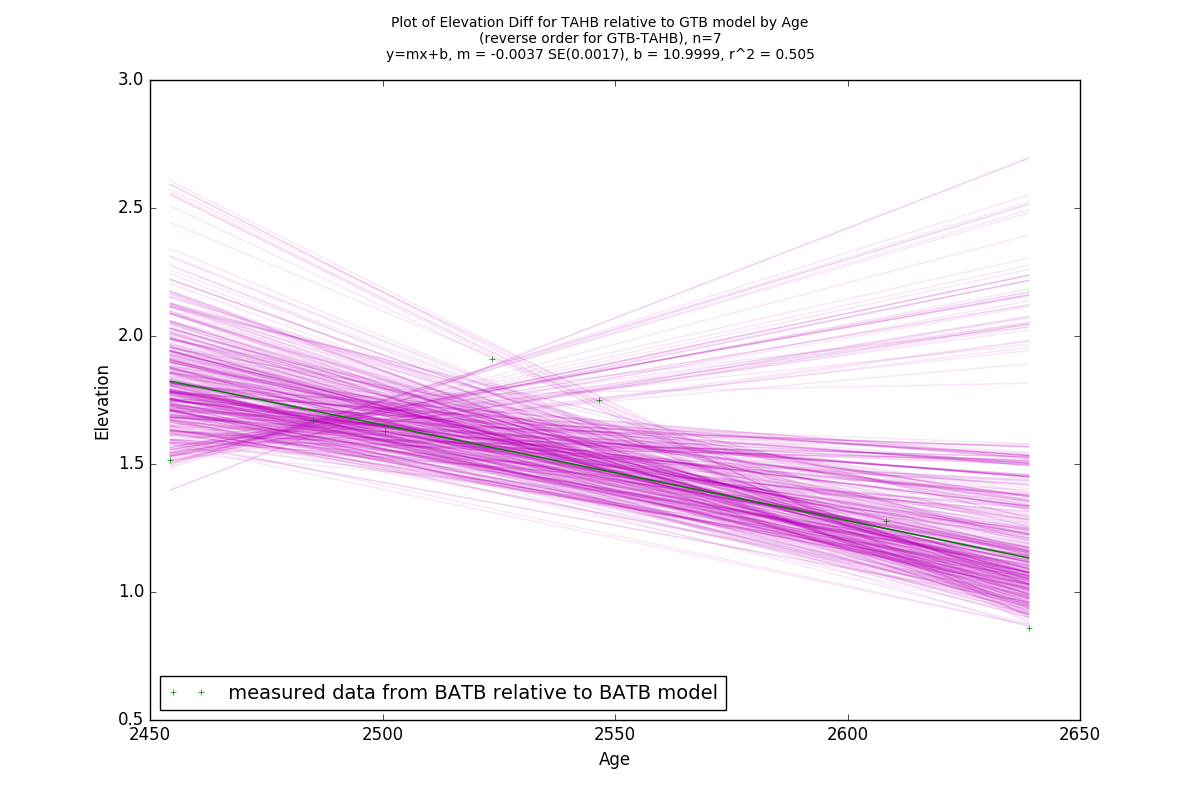
\includegraphics[width=0.9\linewidth]{data/gias/theGIA_TAHB_relative_to_GTB.png}
	\caption{Differences in elevation measured from the TAHB data to the GTB model}
	\label{fig:gias_TAHBxGTB}
\end{figure}
\newpage


\begin{figure}[h]
	\makebox[\textwidth]{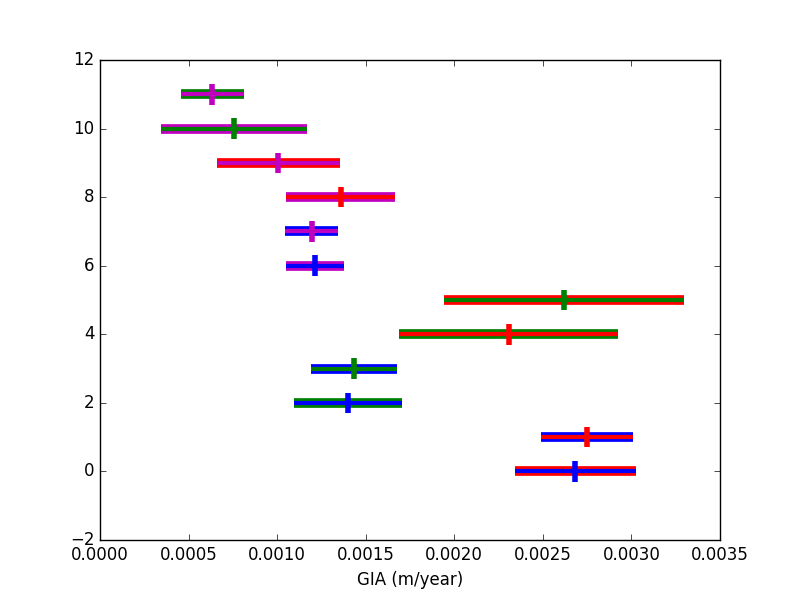
\includegraphics[width=0.6\paperwidth]{data/intervals.png}}
	\caption{95p Confidence intervals on GIA rates obtained from site comparisons}
	\label{fig:intervalsGIA}
\end{figure}


\newpage








\end{document}
